\section{Simulation Study}

This section presents a simulation study evaluating the performance of our proposed estimators on a known data-generating process. The first subsection outlines our simulation study. The section section presents selected results about the bias and mean-square error of our estimators, and the coverage rates for our proposed variance estimation procedure.

\subsection{Study design}

We first generate data according to a known and evaluate the performance of different estimators. For all models we consider the data generating process:

\begin{align*}
Y_{sc} \sim N(X_{1, sc} + X_{2, sc} + X_{3, sc}, \sigma^2_s + \sigma^2_{sc})
\end{align*}

where $\sigma^2_s$ represents the variance component from a state-level random effect, and $\sigma^2_{sc}$ represents a variance component from a CPUMA-level random effect. 

We next define a correlation structure among our observed covariates. Specifically, we generate each covariate vector $X_{sc}$:

\begin{align*}
X_{sc} \sim N(\mu_s, \Sigma_{VV}) \\
\mu_j \sim N(0, \Sigma_{SS}) \\
\end{align*}

Define $Cov(X) = \Sigma_{VV} + \Sigma_{SS} = \Sigma_{XX}$. Let $\sigma^2_{x, j}$ be the j-th diagonal element of $\Sigma_{XX}$ (and define $\sigma^2_{v, j}$ and $\sigma^2_{s, j}$ analogously). Across all simulations, we fix $\sigma^2_{x, j} = 2$. We also fix the off-diagonal elements of both $\Sigma_{XX}$ and $\Sigma_{XX}$ so that $Cor(X_j, X_k) = 0.25$. Finally, define $\rho_x = Cor(X_{sc}, X_{sd})$; in other words, $\rho_x$ is the within-state correlation of $X_{sc}$ (which is constant for each element of $X$).

We also consider there to be $M = 25$ states each with $p_s$ units and $N$ total units. We draw $p_s \sim \lfloor& Exp(0.1) + 10\rfloor$ so that the average number of regions per state is approximately 20 (and the approximate number of total units $N$ is on average approximately 450).

We next generate our noisy outcome and covariate estimates $(J, W)$:

\begin{align*}
(J_{sc}, W_{sc}) \sim N((Y_{sc}, X_{sc}), \Sigma_{\nu\nu, sc})
\end{align*}

\begin{align*}
    \Sigma_{\nu\nu} = \begin{pmatrix}
    \sigma^2_{\nu, sc} & 0 & 0 & 0 \\
    0 & \sigma^2_{\nu, sc} & 0 & 0 \\
    0 & 0 & \sigma^2_{\nu, sc} & 0 \\
    0 & 0 & 0 & \sigma^2_{\nu, sc}
    \end{pmatrix}
\end{align*}

First, define $\rho_y = \sigma^2_{sc}/(\sigma^2_{sc} + \sigma^2_s + \sigma^2_{\nu})$. In other words, $\rho_y$ represents the within-state correlation of the outcome model errors (including the measurement errors).

We allow $\sigma^2_{\nu, sc}$ to be a function of the sample size of an underlying survey that generates the estimate. We simulate these sample sizes $n_{sc}$ drawn from some distribution (see more on this below). Let $N_{sc}$ be a 3x3 diagonal matrix with diagonal elements $n_{sc}$. Let $\sigma_{\nu}^{2\star}$ be defined as the limit as $n \to \infty$ of $n^{-1}\sum_{sc}\sigma^2_{\nu, sc}$ (we ensure this limit exists). Let $\tau = \sigma^2_x/\sigma^2_w$. We then fix a value $\sigma_{\nu}^{2\star}$ so that that as $n \to \infty$, $n^{-1} \tau \sum_{sc}\frac{\sigma^2_{\nu}}{n_{sc}} \to \sigma^2_{\nu}$. In other words, $\sigma_{\nu}^2$ represents the common variance that generate all errors in the ``heterogeneous adjustment'' model. We also simulate homoskedastic measurement errors, letting $\sigma^2_{\nu\nu, sc} = \sigma^2_{\nu\nu}$. 
For our simulations we generate population datasets of $M = 5000$ that consider all 54 combinations of the following parameters:

\begin{itemize}
    \item $(n_{sc} \sim Unif(300, 2300), n_{sc} = 1)$ 
    \item $\rho_x \in \{0, 0.25, 0.5\}$
    \item $\tau \in \{0.95, 0.9, 0.85\}$
    \item $\rho_y \in \{0, 0.25, 0.5\}$
\end{itemize}

For each data parameterization we take 250 random samples of size $M = 25$ and estimate H-SBW weights with targeting $\upsilon_0 = c(1, 1, 1)$. We set $\delta = 0$ and consider $\rho \in \{0, 0.25, 0.5\}$. We then estimate weights balancing on the following datasets: ($W$, $X$, $\hat{\eta}^{HOM}(W))$, $\hat{\eta}^{HET}(W)$) where HOM and HET represent the homogeneous and heterogeneous adjustments. We estimate the variance for each estimator using the leave-one-state-out jackknife, described in Section~\ref{sec:methods}. 
 
Note: for $\hat{\eta}$ we use the empirical covariance matrix of $W$, the estimated means $\bar{W}$, and $\hat{\Sigma}_{\nu\nu, sc}$, where we draw $\hat{\Sigma}_{\nu\nu, sc}$ from $\Sigma_{\nu\nu, sc} + N(0, 0.001*N*I_d)$. In other words, when averaged together we assume that $\hat{\Sigma}_{\nu\nu}$ have a fairly precise estimate of $\Sigma_{vv}$.

\subsection{Selected results}

We present selected results from this study. We consider parameterizations where $\rho_y = 0.25$ and the measurement error variances are heterogeneous (ie the ``heterogeneous adjustment'' model is correct). Figure XX displays the bias associated with each estimator. From left to right, the panels reflect different values of $\tau = \sigma^2_x/\sigma^2_w$ -- the left-most panels have the most measurement error while the right-most panels have the least. From top to bottom the panels reflect different values of $\rho_x$: the top-most panel has no correlation structure among the covariates, while the bottom-most panels are more highly correlated within state. Within each panel we organize each result by which covariate set was balanced: $W$ represents the estimators generated without any covariate adjustment; $X$ reflects estimators generated on the true covariates; $Xhat-het$ represents the heterogeneous adjustment, and $Xhat-hom$ represents the homogeneous adjustment. The estimators are colored by the assumed value of $\rho$ in the H-SBW objective: across all simulations, the true $\rho$ for the outcome model ($\rho_y$) is again 0.25.

We highlight a few interesting results from this plot. First, balancing on $W$ results in bias, and the bias increases with as $\tau$ decreases. Moreover, when all of the covariates are uncorrelated (ie the top panel), balancing on $X$, $Xhat-het$, or $Xhat-hom$ results in approximately unbiased estimates for all values of $\rho$. This aligns with our theoretic results in Appendix A Section I. However, we also see that when $X$ are correlated, setting $\rho > 0$ results in biased estimates for $Xhat-het$ or $Xhat-hom$. On the other hand, if we know the true values of $X$, H-SBW still results in an unbiased estimate. This also aligns with our results in Appendix A, Sections II and III. However, the bias from H-SBW is still much less than the bias for the corresponding estimates that balance on $W$. 

\begin{figure}[H]
\begin{center}
    \caption{Simulation study: estimator bias}
    \label{fig:loveplotc1}
    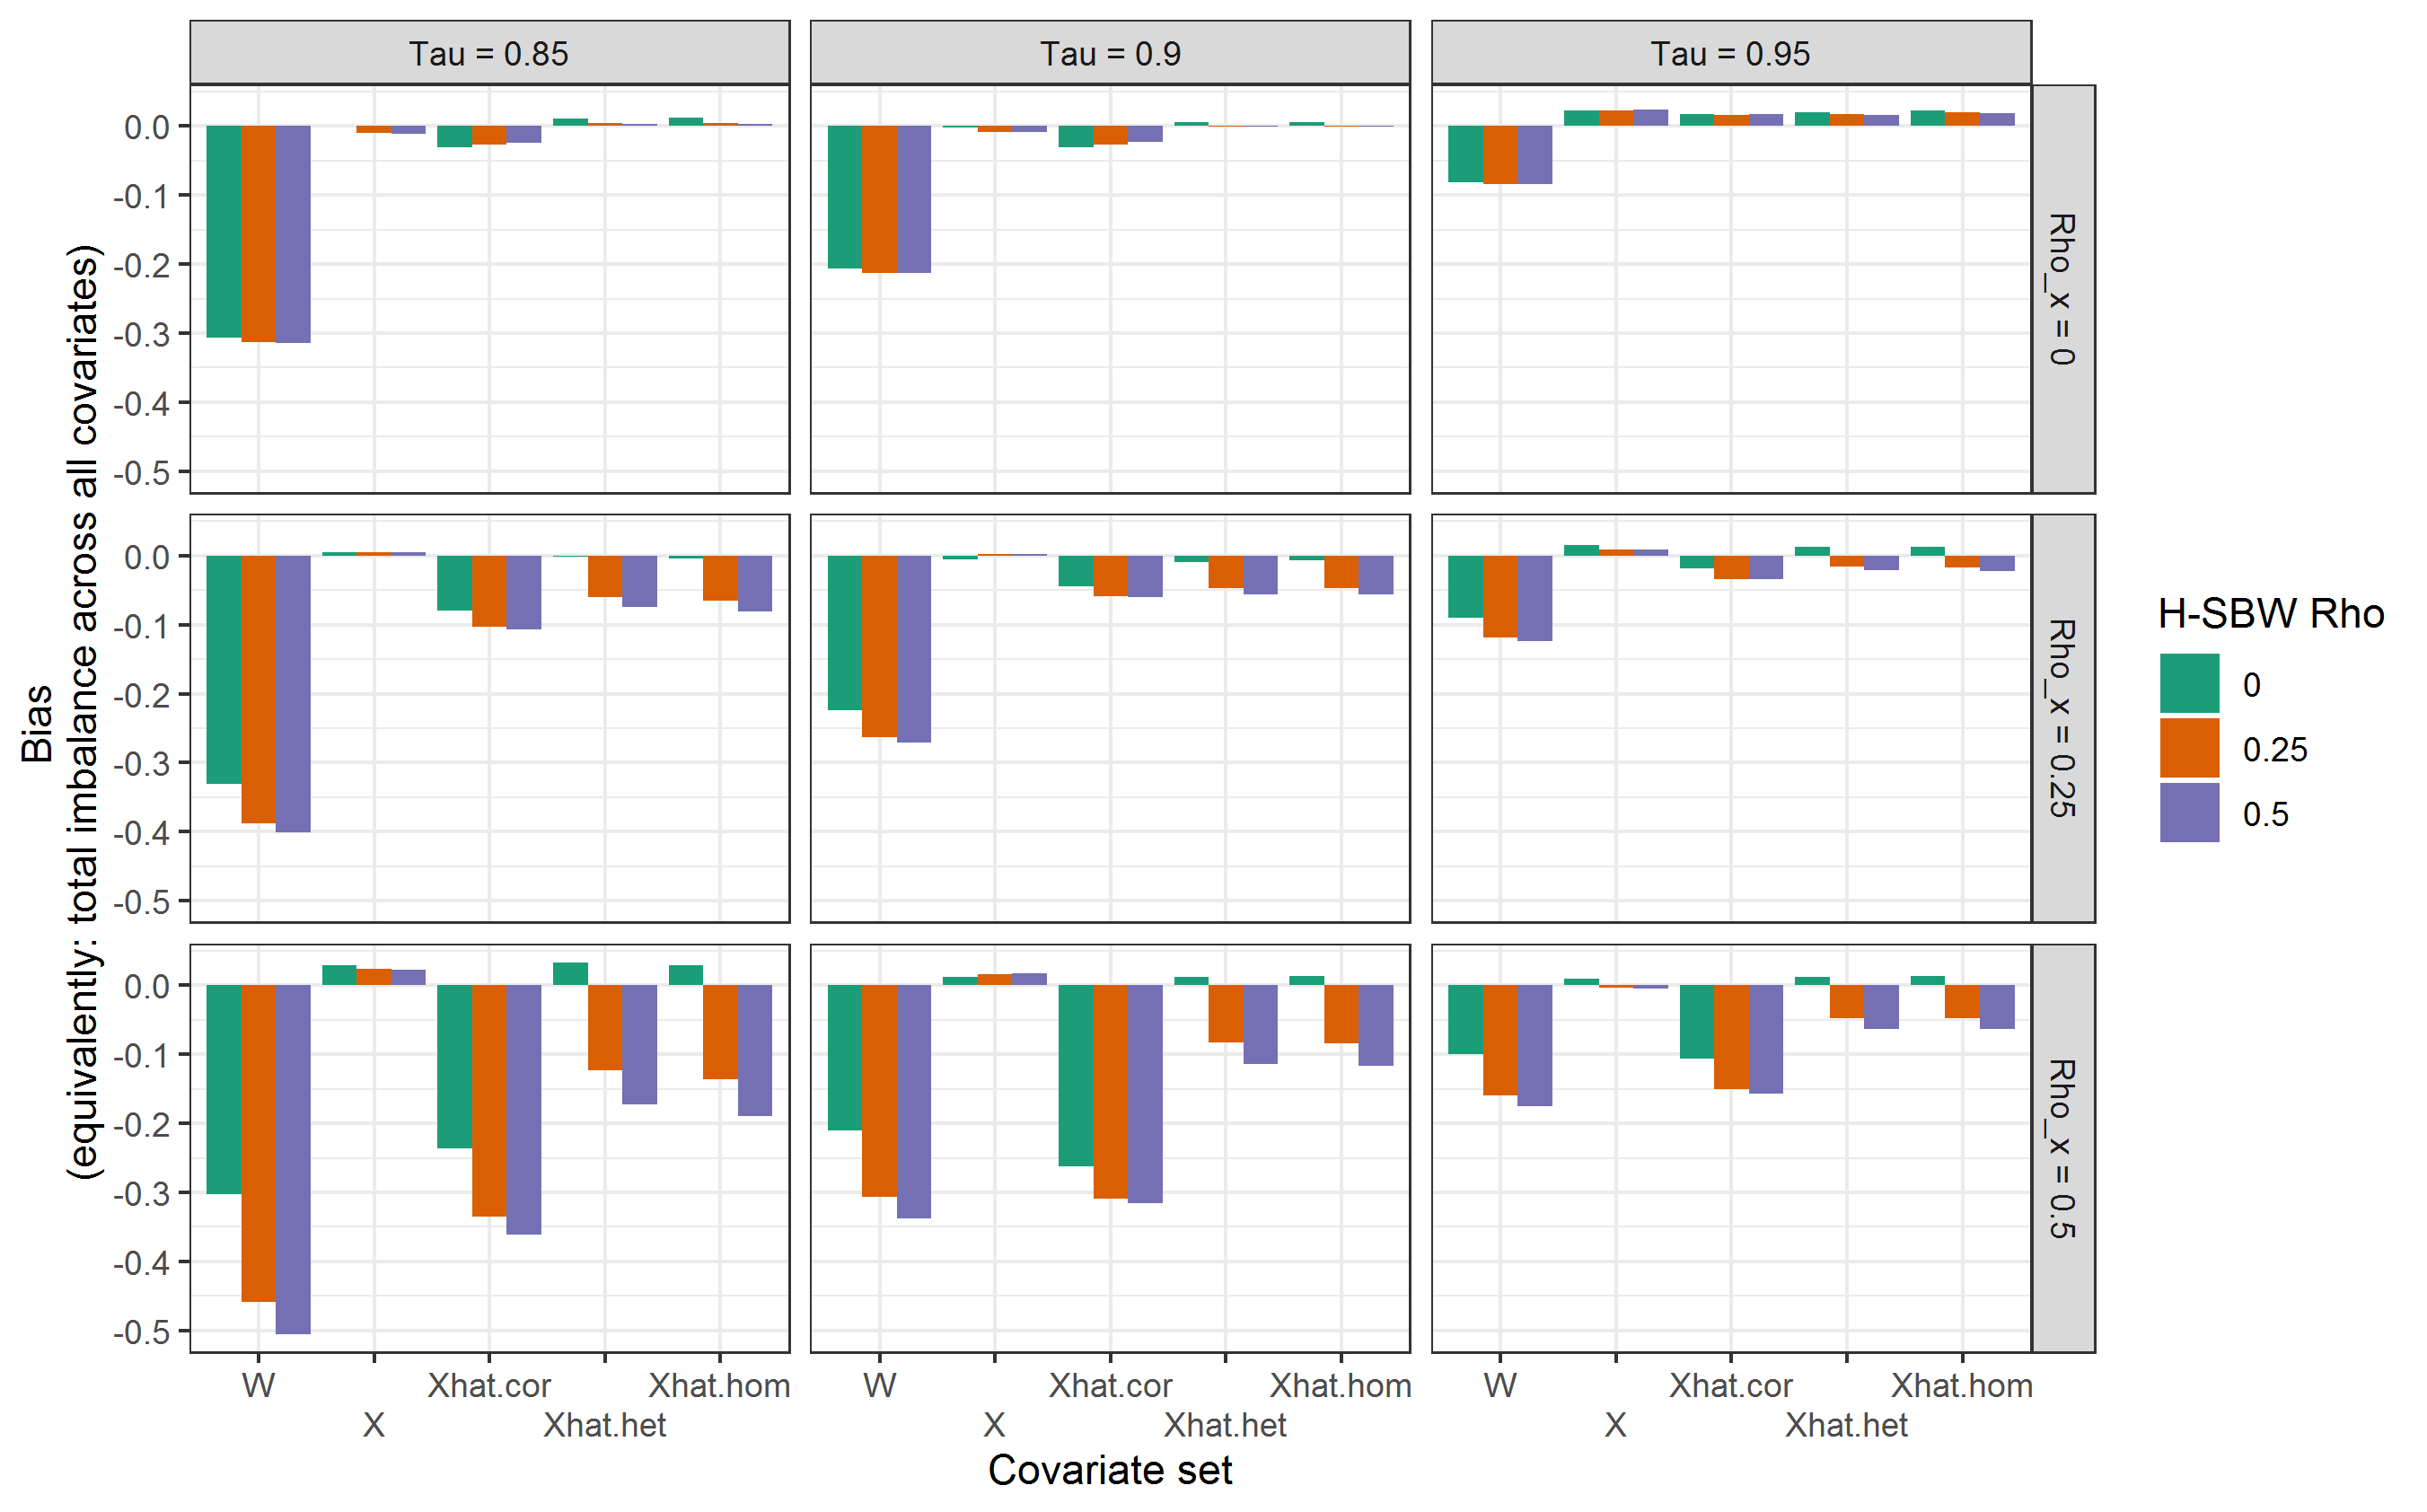
\includegraphics[scale=0.5]{01_Plots/bias-plot.png}
    \subcaption{Averaged across 250 simulations for each specification}
\end{center}
\end{figure}


These estimates are all assuming that the measurement errors are heterogeneous. When we examine the results when the errors are homogeneous, we find that the heterogeneous adjustment has a small bias even when $\tau = 0$ or $\rho = 0$ (results available on request). Assuming this model is correct when it is not therefore appears to have some cost. This may help explain the worse performance we found in for the heterogeneous adjustment in our study in Section~\ref{ssec:allresults}.

We next calculate the standard deviation of the observed estimates. Figure YY displays these results. Unsurprisingly, we find that we obtain a modest variance reduction as we increase $\rho$. Interestingly, even when $\rho$ is incorrect (assumed $0.5$ instead of $0.25$), we tend to much better than when assuming $\rho = 0$, and the performance is in general comparable between $\rho = 0.25$ and $\rho = 0.5$.

In Figure XX we display the MSE of these estimators. We find that despite the increase in bias for $H-SBW$ on the $Xhat-het$ and $Xhat-hom$, we still find a modest reduction in the MSE for many parameterizations. The few exceptions appear to occur when $\tau$ is low and $\rho_x$ is high. These results are consistent with our theoretic results in Appendix A, Section III, which show of these factors tend to accentuate the bias induced by $H-SBW$.

Finally, we evaluate the performance of the leave-one-state-out jackknife procedure and evaluate confidence interval coverage. When $\rho_y = 0$ we find that we obtain approximately nominal coverage rates across all specifications that use $X$ or some version of $\hat{X}$. However, we fail to get even close to nominal coverage rates when balancing on $W$, even when $\tau$ is quite high. We do see the performance of our estimates deteriorate as we increase $\rho_x$, even when balancing on the true covariates. We also see that our coverage rates tend to get worse for $\hat{X}^{het}$ and $\hat{X}^{hom}$ in the settings where we found the highest bias.

The figure displays one final and subtle but interesting feature: when we observe $X$, setting $\rho > 0$ appears to improve the coverage rates. We speculate this may be because H-SBW more evenly dispersing weights across states, increasing the ``effective sample size'' of the states, and thereby improving the asymptotic approximation of the variance estimates. 

The previous analysis takes the covariate adjustment as given. We therefore should expect -- and we do find -- that we get slightly smaller than nominal coverage rates because we haven't accounted for the variability in the adjustment estimates. We therefore conclude by conducting the same procedure but recalculating the covariate adjustment at each state in the leave-one-state out estimates, and we compare the results in Figure XX below.

As expected, we see that our coverage rates increase; however, we often find that our inference is often conservative in regimes where we expect the estimates to be unbiased. When the estimates are biased, we still often fail to achieve nominal coverage rates though even in the worst cases for either variance estimates we do not fall below 85 percent coverage rates.

The results are similar when considering $\rho_y \in \{0, 0.5\}$ and considering homoskedastic measurement errors. One interesting takeaway throughout is that our simulations do not find much evidence that the ``heterogeneous adjustment'' results in much improvement of our estimates, even in an ideal setting. A second interesting finding is that while $\rho > 0$ can bias our estimates in the context of measurement error, the bias is generally small relative to the bias of balancing on the noisy covariate measurements $W$. Of course, this simulation study assumes throughout that we know the true data generating model. 

